\section{Compiling data-plane algorithms}
\label{s:compiler}

\begin{figure}
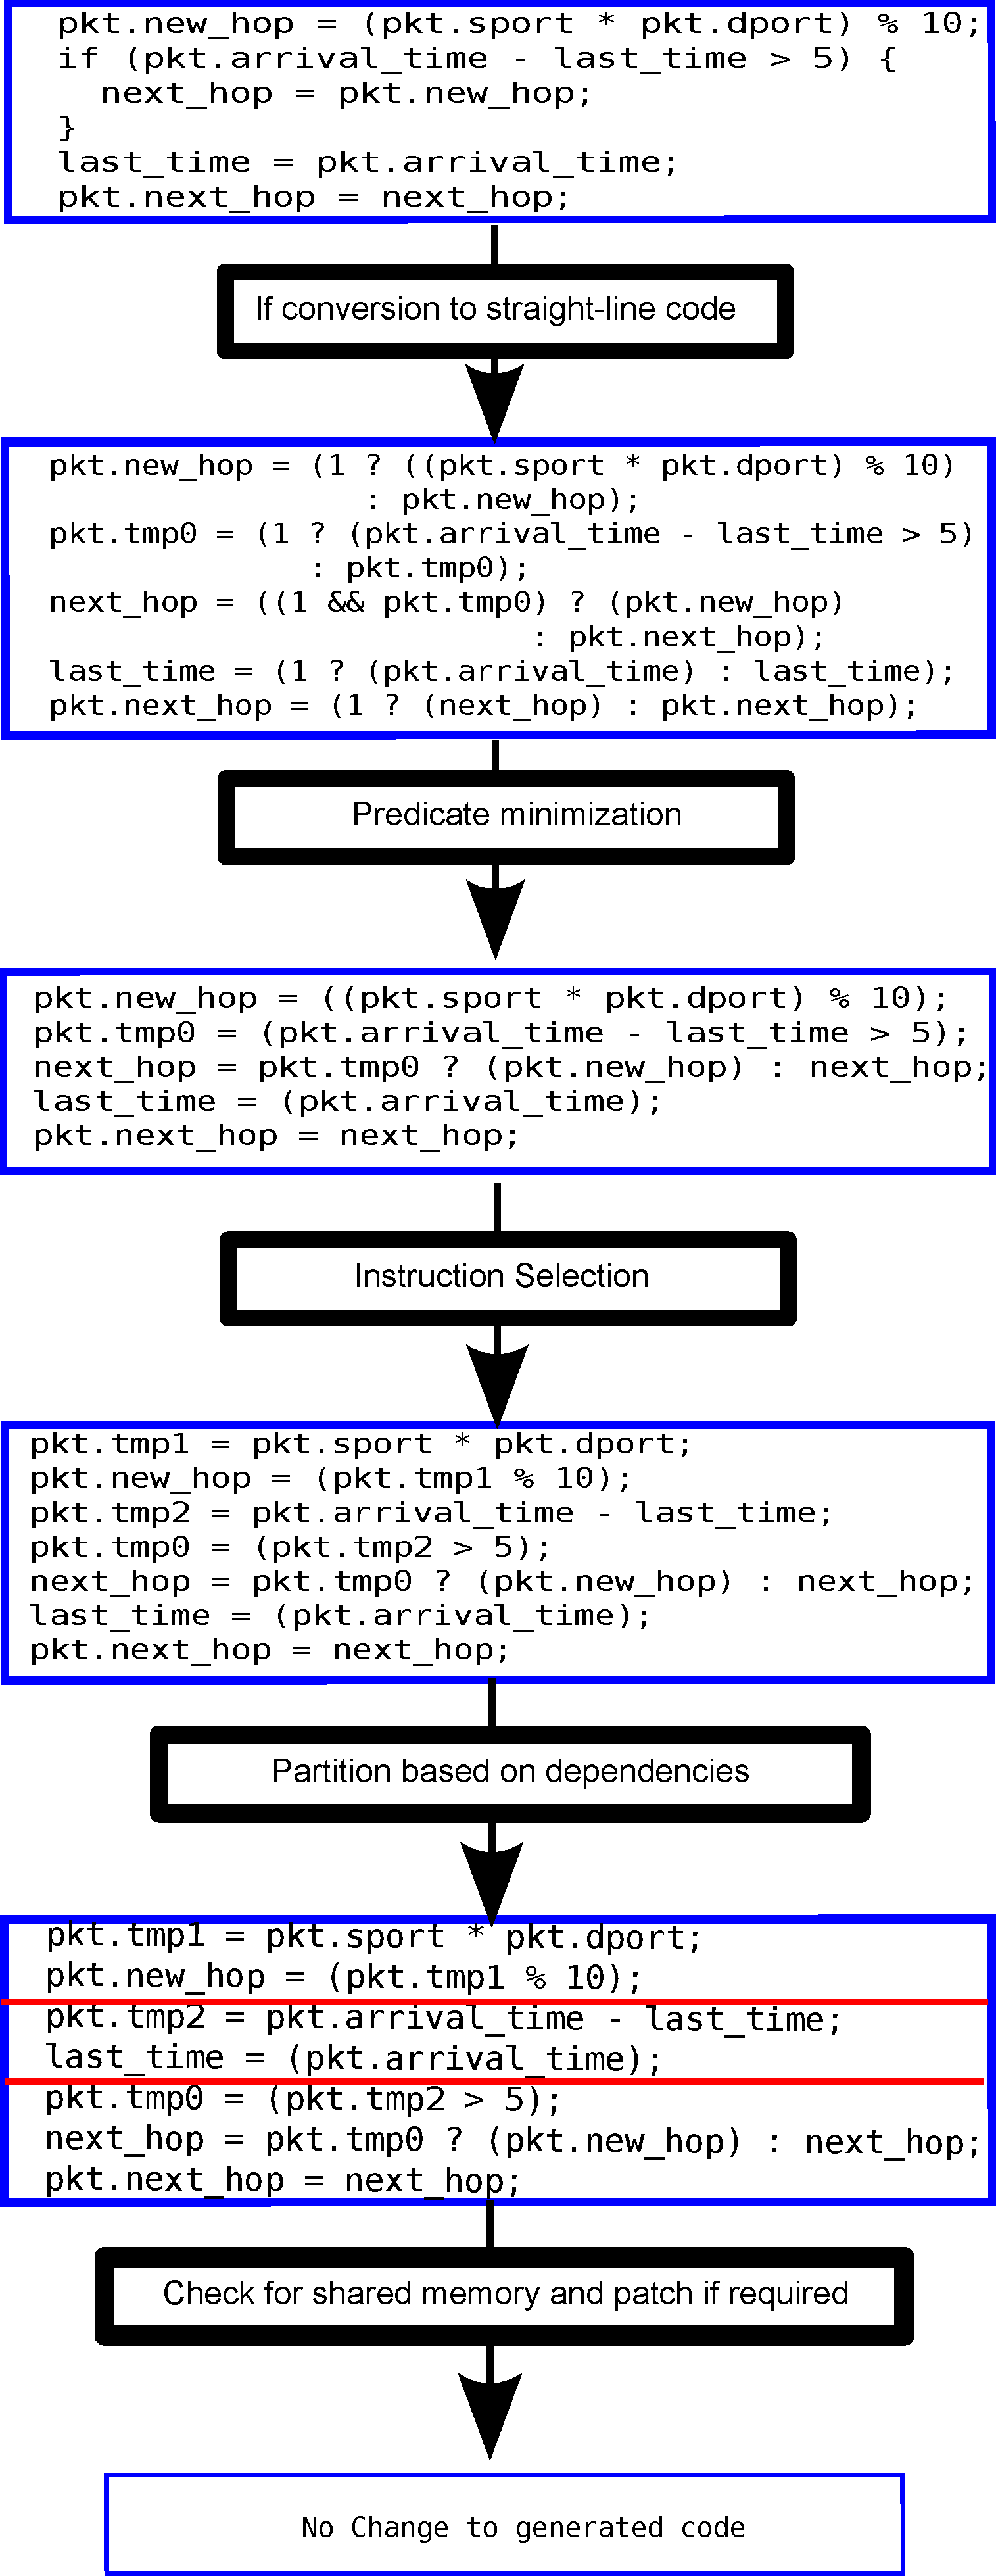
\includegraphics[width=\columnwidth]{compiler_flow.pdf}
\caption{The flow of code through the compiler}
\end{figure}

We next present the design of a compiler that takes code written in \pktlanguage{}
and produces code that can be executed on a pipelined switch architecture, such
as the RMT model~\cite{rmt}. The target code needs to be specified on a a
per-stage basis, while respecting the semantics of the original transactional
specification.  Figure~\ref{fig:flow} provides a high-level overview of
the input and output to the compiler for the running example that we use
throughout this section: load balancing using flowlet
switching~\cite{dina_flowlets}.

For ease of exposition, our target language is syntactially identical to our
source language, but differs semantically in a few key ways to match the
hardware. First, statements within a stage execute in parallel. Second,
statements within a stage map 1:1 with hardware op codes. Third, control flow
is disallowed within a stage.

Recall from \S\ref{s:dataplane} that these are exactly the characteristics that
distinguish \pktlanguage{} from P4. In the future, we plan to implement our
compiler as a source-to-source translator that translates \pktlanguage{} to P4.
This allows us to leverage existing work on P4
compilation~\cite{lavanya_compiler, brebner, netronome} that translates P4 to
the register configuration of the target architecture.

We structure the compiler as a sequence of passes and describe each of them in
turn below. 

\subsection{Turning packet variables into local variables}
As a first step, the compiler transforms packet attributes (syntactically
repsented as C member variables) into local variables.  This is a correct
transformation because packet variables are only alive through the duration of
the function body. Implementing this is straightforward: we scan the Abstract
Syntax Tree (AST) of the source code looking for the C member of object
operator and replace it with a local variable, prepending a declaration to the
source code.

\subsection{Converting to straight-line code}
A general transaction body can contain convoluted control flow using if-else
statements. As an extreme example, consider the source code for CoDel:
\url{http://queue.acm.org/appendices/codel.html}. Control flow complicates
dependence analysis. We eliminate control flow by transforming if-else
statements using the ternary operator, starting from the innermost if
statements and recursing outwards using a well-known procedure called if
conversion~\cite{allen_if_conversion}. At the end of this pass, we also
simplify the predicates used in the ternary operator if possible. This
transformation creates straight-line code, where control always passes from one
statement to the next without any branching.

\subsection{Instruction Selection}
We next replace portions of the straight-line code with code that maps 1:1 to
the underlying hardware. As a contrived example, if the underlying hardware
supports read and write operation on stateful memory, but does not support
atomic increment operations on stateful memory, we would have to replace the
statement: \texttt{x = x + 1;} with three statements:
\begin{verbatim}
int tmp1 = x;
int tmp2 = tmp1 + 1;
x = tmp2;
\end{verbatim}

Other more involved examples of instruction selection include ``flattening''
expressions~\cite{expression_flattening} with deep ASTs into a canonical form
where the right hand side of each assignment is a simple expression that
doesn't contain any expressions within it. These simple expressions would then
map 1:1 to underlying hardware constructs.

\subsection{The one-packet compiler}
After instruction selection, the resulting straight-line code maps 1:1 to the
underlying hardware. At this stage, the code is correct if executed in a
straight-line assuming exactly one packet ever executes the code. A
straightforward partitioning simply assigns each instruction to a separate
stage, but is wasteful. Many instructions may have no dependencies between them
and can be executed in parallel.

To determine a better partitioning, we first scan every pair of instructions
to determine if they can be executed in parallel. Two instructions can be
executed in parallel (and hence moved into the same stage) as long as:
\begin{enumerate}
\item They don't write to the same variable.
\item One instruction doesn't read a variable written by the other.
\end{enumerate}
We start by assigning the first instruction to its own stage. We then go
through the remaining instructions sequentially, assign each one to the
earliest stage where it can execute in parallel with all instructions in that
stage, and create a new stage every time such a stage does not exist.
%TODO: We need to fix this. I am not sure exactly what the algorithm is.

%%TODO: Might write if we have space.
%%This approach does not take into account constraints on the number of parallel
%%actions that can execute within a single stage. Action constraints depend on
%%other features (such as ACLs, routing tables, tunelling tables) that share the
%%same stage.  Whis is best handled
%%one layer lower, where the P4 code fragment 
%%

\subsection{Detecting memory sharing across stages}
In our entire discussion so far, we make no distinction between stateful
variables and packet-local variables. This is because, if there is only a
single packet in the system, there is no distinction between the two.

In this pass, we scan the partitioning created by the one-packet compiler,
looking for stateful variables (any globally declared variable), and checking
if any stateful variable is read in one stage and then written in a subsequent
stage. If this is the case, that stateful variable needs to be shared across
stages and the best we can do is to approximately emulate such sharing using
recirculation.

Instead, if a stateful variable is written in exactly one stage, but read in
multiple stages following the stage that it is written in, we can achieve this
effect by simply writing the stateful variable into a packet field that then
carries the value to subsequent stages.

We note here that this pass relies on the instruction selection pass to
determine a good set of instructions that map closely to the hardware. For
instance, if instruction selection cannot rewrite the set of sequential
statements: \texttt{x = x + y; y = y + x;} into the tupled form \texttt{(x, y)
= (x + y, 2 * y + x);}, then the one-packet compiler will move \texttt{y = y +
x;} into the stage following \texttt{x = x + y;} causing spurious memory
sharing.

\subsection{Patching code to achieve memory sharing}

\subsection{Translating to P4}
As a final step, we translate the partitioned code (patched, if required)
into P4. This is a conceptually straightforward process:
\begin{enumerate}
\item We add newly created temporary variables to the header and parser
specifications so that P4 can automatically generate the parser state machine.
\item We create a P4 logical table for each partition.
\item The set of packets on which the algorithm will run is specified using
an appropriate match type (exact, ternary, or longest-prefix) on specific
header fields within each logical table.
\item We create a P4 action in each logical table from the code in the
corresponding partition.
\item Lastly, the control-flow between P4 tables mirrors the order of
partitions.
\end{enumerate}

%Advanced idioms:
%--> Pipeline wide memory using recirculation primitive.
%--> Tupled Stateful operations: <x, y> <--- f(x, y).
%--> Multiply accumulate (MAC).
%
